
% Options for packages loaded elsewhere
\PassOptionsToPackage{unicode=true}{hyperref}
\PassOptionsToPackage{hyphens}{url}
%
\documentclass[a4paper]{article}
\usepackage{lmodern}
\usepackage{amssymb,amsmath}
\usepackage{mathtools}
\usepackage{geometry}
\geometry{a4paper, left=25mm, right=25mm, top=25mm,bottom=25mm}
\usepackage{url}
\usepackage[T1]{fontenc}
\usepackage[utf8]{inputenc}
\usepackage{textcomp} % provides euro and other symbols
\bibliographystyle{siam}
\setlength{\parindent}{0pt}
\setlength{\parskip}{6pt plus 2pt minus 1pt}
\usepackage{xcolor}
\usepackage{hyperref}
\usepackage{color}
\usepackage{fancyvrb}
\usepackage{algpseudocode}
\usepackage{algorithm}
\usepackage{graphicx,grffile}
\usepackage{subcaption}
\usepackage{float}
\usepackage{courier}
\usepackage{jlcode}
\usepackage{minted}

\title{DPMM.jl}
\author{
  Ekin Akyürek\\
   CSAIL, Massachusetts Institue of Technology\\
   Koç University\\
  \texttt{akyurek@mit.edu}
 }



\begin{document}
\maketitle

\section{Introduction}

This repository is a research work on parallel dirichlet process mixture
models and clustering on Julia by Ekin Akyürek with supervision of John
W. Fischer III.

\section{Bacground}

\subsection{Mixture Models}

Mixture models are statistical models for representing a data comes from
different probability distributions. A mixture model generally
parametrized by mixture(i.e component) parameters and mixture weights
which can be considered as prior probability of mixtures in the Bayesian
setting. The more weight attached to a mixture, the more data comes from
that mixture. In this work, we will mostly use the notation for mixture
models which are presented in the document\cite{kamper2013gibbs}:

\paragraph{Data}
\begin{center}
\begin{tabular}{|l|l|}
\hline
$N$ & Number of data vectors \\
$D$ & Dimension of data vectors \\
$x_i \in R^D$ & The $i^th$ data vector \\
$X = (x_1, x_2,...,x_N)$ & Set of data vectors \\
$X_{\setminus i}$ & Set of data vectors, without taking $x_i$ into account\\
$X_k$  & Set of data vectors from mixture component $k$ \\ 
$X_{k \setminus i}$  & Set of data vectors from mixture component $k$, without taking $x_i$ into account  \\
$N_k$ & Number of data vectors from mixture component $k$ \\  
$N_{k \setminus i}$ & Number of data vectors from mixture component $k$, without taking $x_i$ into account \\ \hline
\end{tabular}
\end{center}

\paragraph{Model}
\begin{center}
\begin{tabular}{|l|l|} \hline
$K$ & Number of components in a finite mixture model \\
$z_i$ & discrete latent state indicating which component observation $x_i$ belongs to \\
$\mathbf{z} = (z_1, z_2,...,z_N)$ & Latent states for all observations $x_i,..., x_n$\\
$\mathbf{z}_{\setminus i}$ & Set of all latent states excluding zi\\
$\theta_k$  & Component parameters (e.g. $\mu_k$, $\Sigma_k$ in a gaussian mixture model)  \\
$\pi_k$ & Prior probability that data vector $x_i$ will be assigned to mixture component $k$ \\
$\mathbf{\pi} = (\pi_1,\pi_2,...,\pi_K)$ & Prior assignment probability for all $K$ components \\
$\beta$ & Hyperparameters of the prior distribution for $\theta$ parameters in a bayesian setting \\ \hline
\end{tabular}
\end{center}


\subsection{Dirichlet Process Mixture Models (DPMM)}

\subsubsection{Dirichlet Processes (DP)}

There are many ways to interpret DP. Formally, it is random process
whose realizations are probability distributions. The constructive
definition of dirichlet process is done by stick-breaking processes.
Chineese Restraunt Process(CRP) and Pólya Urn Scheme also leads to DP.
All these definitions are related with each other thanks to
\href{https://en.wikipedia.org/wiki/De_Finetti\%27s_theorem}{de
Finetti's exchangibility theorem}.

DP is parametrized by \(\alpha\) concentration parameter and \(G_0\)
base distribution. One can show that \(\alpha\) controls how similar
draws to the \(G_0\). Therefore, G is used to denote samples drawn from
DP.


\subsubsection{Stick-Breaking Construction}

Stick-breaking provides a nice way to draw samples from, but it requires
to countably infinite summation. As we stated earlier, draws from DP is
itself a distribution which is indeed discrete. Stick-Breaking steps are
deliniated in the below.

\begin{align*}
v_1,v_2,...,v_i,... & \sim Beta(1,\alpha) \\
\pi_i &= v_i \prod_{j=1}^{i-1}(1-v_j) \\ 
\theta_1,\theta_2,...,\theta_i,... & \sim G_0 \\
G & = \sum_{i=1}^{\infty}\pi_i\delta_{\theta_i}
\end{align*}

Here \(\delta_{\theta_i}\) is a indicator function centered on
\(\theta_i\), namely \(\delta_{\theta_i}(\theta)\) is zero everywhere
except \(\theta=\theta_i\). Realize that \(\pi_i\)'s approaches to zero
as i goes to infinity, so it enables to approximate G using a finite
summation instead of infinite one.


\subsubsection{Chineese Restraunt Process (CRP)}

Chineese restraunt process is a dicrete process which is named after the
analogy of seating customers to at tables in a restraunt. Let say
customers \(1:N\), we will seatch each customer sequentially with the
following probabilities where \(c_k\) is the number of customers seated
\(k^{th}\) table and, \(i\) is current number of customers seated in the
restraunts.
\begin{equation*}
z_i|z_1,...,z_{i-1} = \begin{cases}
P(z_i=k)=\frac{c_k}{i-1+\alpha} & \text{for an existing table} \\
P(z_i=K+1)=\frac{\alpha}{i-1+\alpha} & \text{for opening a new table}
\end{cases}
\end{equation*}

Note that this proceess is independent of the order of customers. This
means that the CRP is exchangable\cite{fang2016dirichlet}.

If we assuma a base measure \(G_0\) as a prior for table/cluster
parameters and assign each table a probability measure sampled from
\(G_0\), the process becomes CRP Mixture Model or Pólya Urn Scheme.

\begin{align*}
\theta_1...,\theta_K,... &\sim G_0 \\
z_i|z_1,...,z_{i-1} &= \begin{cases}
P(z_i=k)=\frac{c_k}{i-1+\alpha} & \text{for an existing table/cluster} \\
P(z_i=K+1)=\frac{\alpha}{i-1+\alpha} & \text{for opening a new table/cluster}
\end{cases}\\
X_i|z_i &\sim f(X_i|\theta_{z_i})
\end{align*}

Exchangibility allows us to show that above model equals to\cite{blackwell1973ferguson}:

\begin{align*}
G &\sim DP(\alpha,G_0)  \\
\theta_i|G &\sim G \qquad i \in 1,...,N \\
X_i|\theta_i &\sim  f(X_i|\theta_i) \qquad i \in 1,...,N \\
\end{align*}

\subsubsection{Formal Definition}

We stated that samples from dirichlet process were probability
distribution itself. Let say a sample is a probability distribution over
S space. Let \(\{A_i\}_{i=1}^n\) denote a measurable partition of S. For
any measureble partition of S below statement holds (\(Dir\) is
Dirichlet Distribution):

\begin{equation*}
G \sim DP(\alpha,G_0) \implies  (G(A_1),G(A_2),...,G(A_N)) \sim Dir(\alpha G_0(A_1),...,\alpha G_0(A_N))
\end{equation*}

This defines Dirichlet Process, however doesn't allow to draw samples
from unlike CRP or Pólya Urn.


\subsubsection{Infinite Mixture Models}

As we show in CRP section, Diricihlet process is very good prior on
cluster parameters because we can model infinite number of clusters.
Note that every finite data realization of DPMM is a finite mixture
model with Dirichlet distribution as shown in formal definition. One can
use finite stick-breaking process to construct DP, however it has
approximation errors. On the other hand, CRP Mixture Model provides
exact way to sampling or do inference on the mixture data. Finally,
these two different representations are summarized by below graphical
model representations. In the following section we will discuss how to
do inference on DPMM.

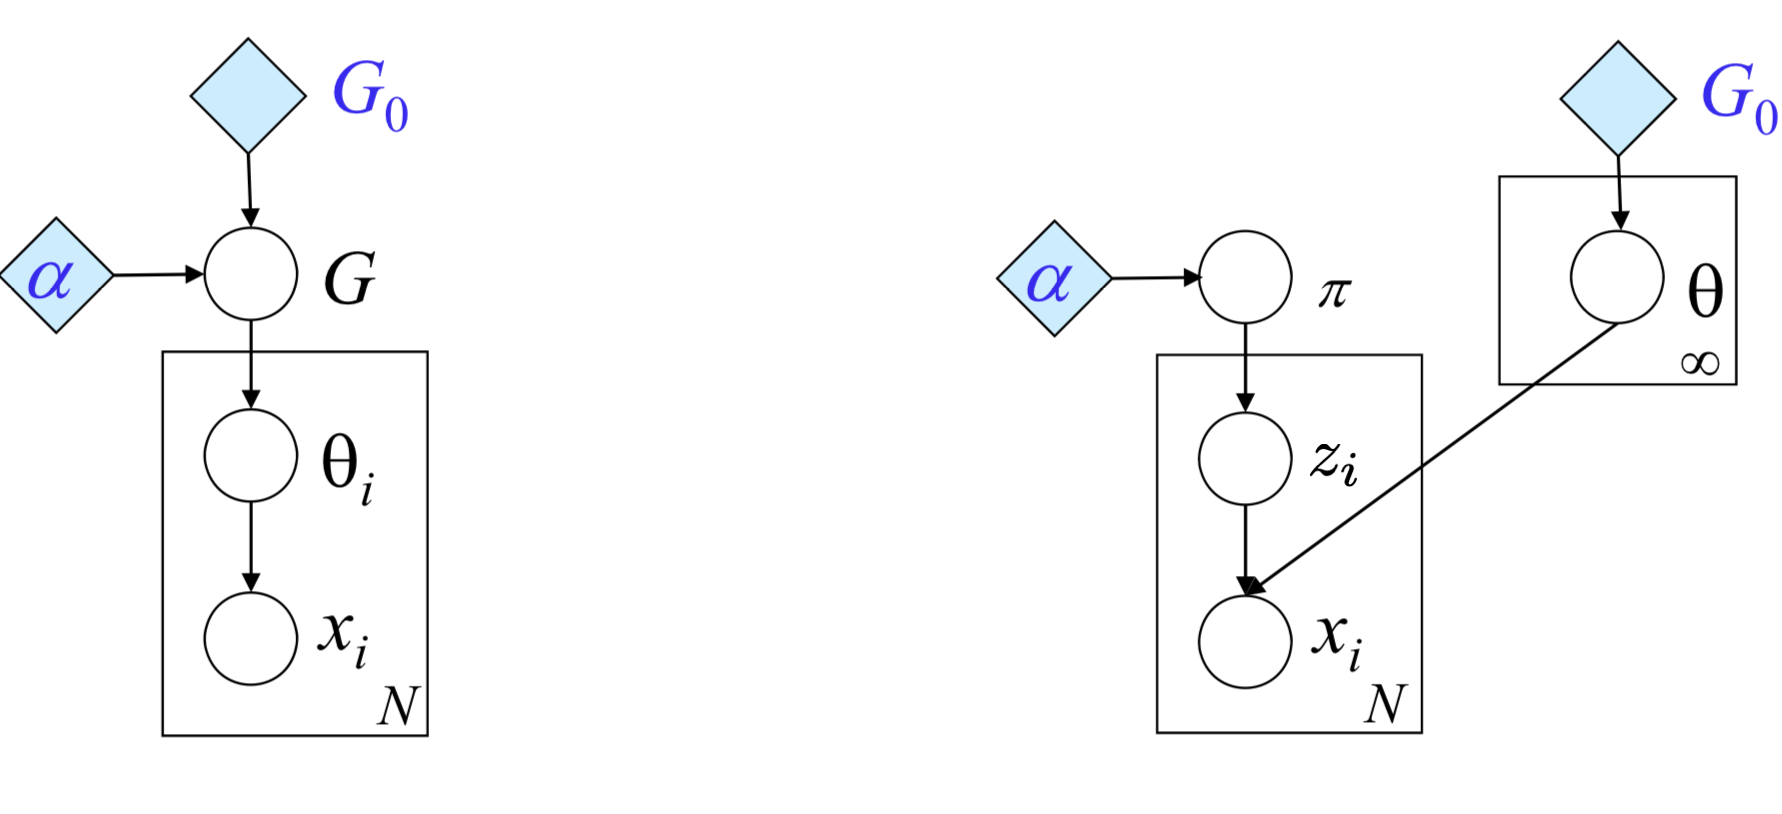
\includegraphics[width=\textwidth]{img/pgm-dpgmm.png}

\subsection{Inference in DPMM}

Inference problem that we interested is to obtain cluster assignments
for each data point given base distribution \(G_0\) and \(\alpha\)
parameter. We will use conjuagte prior which assure that posterior
probability of cluster parameters are in same distribution family with
the prior. Let's investigate conjugate priors for Gaussian and
Multinomial distributions.


\subsubsection{Gaussian Conjugate: Normal-Inverse-Wishart Distribution}

Multivariate Gaussian Distribution generally parametrized by mean vector
\(\mu\) and covariance matrix \(\Sigma\). Normal-Inverse-Wishart(NIW)
Distribution\cite{murphy2007conjugate} is the prior distrubution for Gaussian with unkown \(\mu\) and and
unknown \(\Sigma\).

Normal-Inverse-Wishart is parametrized by:

\begin{center}
\begin{tabular}{|l|l|}
\hline
 $\boldsymbol \mu_0$  & prior mean for $\mu$ \\ 
 $\boldsymbol \Psi_0$ & proportional to prior mean $\Sigma$\\
 $\lambda_0$ & how strongly we believe the  $\mu_0$\\
 $\nu_0$ & how strongly we believe the  $\Psi_0$\\ 
 \hline
\end{tabular}
\end{center}

NIW has seperable pdf function with Gaussian and
Inverse-Wishart(\(\mathcal{W}^{-1}\))
\begin{equation*}
p(\boldsymbol\mu,\boldsymbol\Sigma|\boldsymbol\mu_0,\lambda_0,\boldsymbol\Psi_0,\nu_0) = \mathcal{N}\left(\boldsymbol\mu\Big|\boldsymbol\mu_0,\frac{1}{\lambda}\boldsymbol\Sigma\right) \mathcal{W}^{-1}(\boldsymbol\Sigma|\boldsymbol\Psi_0,\nu_0)
\end{equation*}
The \(\mathcal{W}^{-1}\) includes \texttt{inverse} because the inverse
of the sampled matrices has Wishart(\(\mathcal{W}\)) distrubition. To
understand further and to learn how to sample from Wishart distribution
see the reference for the Bartlett decomposition method \cite{wishart1928generalised}.

If we use sample mean(\(\hat{\mu}\)) and sample
covariance(\(\hat{\Sigma}\)) matrix as sufficent statistics, posterior
parameters for the Normal-Inverse-Wishart distribution is given by the
below equations\cite{kamper2013gibbs}:

\begin{align*}
p(\boldsymbol\mu,\boldsymbol\Sigma|\mathcal{X}) & = NIW(\boldsymbol\mu,\boldsymbol\Sigma| \boldsymbol  \mu_N,  \boldsymbol  \Psi_N, \lambda_N, \nu_N)  \\
\boldsymbol \mu_N & = \lambda_0 \boldsymbol \mu_0 + N \hat{\mu} \\
\lambda_N & = \lambda_0 + N \\
\nu_N & = \nu_0 + N \\
\boldsymbol \Psi_N &=  \Psi_0 + \hat{\Sigma} + \frac{\lambda_0N}{\lambda_0+N}(\hat{\mu}-\boldsymbol \mu_0)(\hat{\mu}-\boldsymbol \mu_0)^T
\end{align*}

It is also possible to store \(t =N\hat{x}\) and \(T=\sum_{i=1}^Nxx^T\)
as sufficient statistics, which is computationally adventagous, the
equations become:

\begin{align*}
\boldsymbol \mu_N & = \lambda_0 \boldsymbol \mu_0 + t \\
\lambda_N & = \lambda_0 + N \\
\nu_N & = \nu_0 + N \\
\boldsymbol \Psi_N &=  \Psi_0 + T + \lambda_0\boldsymbol\mu_0\boldsymbol\mu_0^T-\lambda_N\boldsymbol\mu_N\boldsymbol\mu_N ^T
\end{align*}


\paragraph{\texorpdfstring{Low-Rank Updates for
\(\Psi_N\)}{Low-Rank Updates for \textbackslash Psi\_N}}

In the program we store \(\Psi_N\) cholesky factorized form to sample
efficently. However, we need to calculate cholesk factorization,which is
$\mathcal{O}(n^3)$, everytime if we remove or add single data point.
For that case, there is a faster algorithm to compute updated cholesky
factorization from the previous cholesky factorization\cite{Seeger:161468}. We utilize rank-1
update and rank-1 downdate methods to speed up the collapsed gibbs
sampler.


\subsubsection{Multinomial Conjugate: Dirichlet Distribution}

In discrete data setting, multinomial probabilty distribution is used
for likelihood of data. Dirichlet distribution is the conjugate prior
for multionomial distribution.

TODO


\subsubsection{Collapsed Gibbs Sampler}

When using conjugate priors for cluster parameters, marginal likelihood
of data can be obtained by analytically integrating out the cluster
parameters \(\theta_i\)'s. For the Gaussian parameters the marginal
likelihood:

\begin{equation*}
p(\mathcal{X}) = \int_\mu\int_\Sigma p(\mathcal{X},\mu,\Sigma)p(\mu,\Sigma)d\mu d\Sigma
\end{equation*}

The likelihod of a new data \(x^*\) is given by:
\begin{equation*}
p(x^* | \mathcal{X}) = \frac{p(x^*,\mathcal{X})}{p(\mathcal{X})}
\end{equation*}

It turns out that the posterior likelihood (posterior-predictive) for a
new data has Multivariate Student's t-distribution\cite{kamper2013gibbs}:
\begin{equation*}
    p(x^*|\mathcal{X}) = \mathcal{T}(x^*|\boldsymbol \mu_N,\frac{(\lambda_N+1)}{\lambda_N(\nu_N-D+1)} \boldsymbol\Psi_N,\nu_n-D+1)
\end{equation*}
The inference in DP Gaussian Mixture Models can be done by using CRP
procedure. The difference is that instead of using \(f(x|\theta_{z_i})\)
likelihood, we use \(\mathcal{T}(x|\beta,\mathcal{X_{k \setminus i}})\)
posterior-predictive and we never sample \(\theta\)'s
explicitly \cite{kamper2013gibbs}.

\begin{align*}
z_i|\boldsymbol z_{\setminus i}  &\sim \begin{cases}
P(z_i=k)=\mathcal{T}(x|\beta,\mathcal{X}_{k \setminus i})\frac{N_{k\setminus i}}{i-1+\alpha} & \text{for an existing table/cluster} \\
P(z_i=K+1)=\mathcal{T}(x|\beta)\frac{\alpha}{i-1+\alpha} & \text{for a new table/cluster}
\end{cases}
\end{align*}

Below is the pseudocode\cite{kamper2013gibbs} for collapsed gibbs sampler for DP
Gaussian Mixture Model. Multinomial example can easily be obtained by
changing posterior-predictive in the code.


\begin{algorithm}
  \caption{Collapsed Gibbs sampler for an infinite Gaussian mixture model.}\label{collapsedgibbs}
  \begin{algorithmic}[1]
    
  \State Choose an initial \textbf{z}.
  \For{M iterations} \Comment{Gibbs Sampling Iterations}
    \For{i = 1 to N}
        \State Remove $\mathbf{x}_i's$ statistics from component $z_i$ \Comment{Old assignment for $\mathbf{x}_i$}
        \For{k = 1 to K} \Comment{For all existing clusters}
            \State Calculate $P(z_i = k | \mathbf{z}_{\setminus i},\alpha) = \frac{N_{k\setminus i}}{N+\alpha-1}$ as in CRP
            \State Calculate $p(\mathbf{x}_i|\mathcal{X}_{k\setminus i},\mathbf{\beta})$ using $\mathcal{T}$ distribution above
            \State Calculate $P(z_i = k | \mathbf{z}_{\setminus i},\mathcal{X},\alpha,\mathbf{\beta}) \propto P(z_i = k | \mathbf{z}_{\setminus i},\alpha) p(\mathbf{x}_i|\mathcal{X}_{k\setminus i}, \mathbf{\beta})$
        \EndFor
        \State Calculate $P(z_i = k^* | \mathbf{z}_{\setminus i},\alpha) = \frac{\alpha}{N+\alpha-1}$ as in CRP \Comment{Consider opening a new cluster}
        \State Calculate $p(\mathbf{x}_i|\mathbf{\beta})$ using $\mathcal{T}$ distribution above
        \State Calculate $P(z_i = k^* | \mathbf{z}_{\setminus i},\mathcal{X},\alpha, \mathbf{\beta}) \propto P(z_i = k^* | \mathbf{z}_{\setminus i},\alpha)p(\mathbf{x}_i|\mathbf{\beta})$
        \State Sample $k_{new}$ from $P(z_i = k^* | \mathbf{z}_{\setminus i},\mathcal{X},\mathbf{\alpha},\mathbf{\beta})$ after normalizing
        \State Add $z_i$'s statistics to the component $z_i = k_{new}$.\Comment{New assignment for $\mathbf{x}_i$}
        \State If any component is empty, remove it and decrease K
    \EndFor
  \EndFor
  \end{algorithmic}
\end{algorithm}


\paragraph{Remarks}

\begin{itemize}
\item
  Collapsed sampler is hard to parallelize because in each data point we
  need update cluster statistics, and we don't know which cluster's
  statistic will change beforehand.
\item
  Collapsed sampler has some issues when it starts with under-estimated
  number of cluster. Closer clusters tend to form a single cluster in
  that situation.
\end{itemize}


\subsubsection{Direct Gibbs Sampler}

Another approach for gibbs sampler is direct sampler in which we
explicitly sample \(\theta_k\) by the posterior for each existing
cluster, then we calculate likelihood by cluster's likelihood function.

\begin{align*}
\theta_1...,\theta_K&\sim G_0(\theta|\boldsymbol z, \beta) \\
z_i|\boldsymbol z_{\setminus i} &\sim \begin{cases}
P(z_i=k)= f(X_i|\theta_{k})\frac{N_{k\setminus i}}{i-1+\alpha} & \text{for an existing cluster} \\
P(z_i=K+1)= f(X_i|\theta)\frac{\alpha}{i-1+\alpha} & \text{for a new cluster}
\end{cases}\\
\end{align*}

For each iteration, we repeat these steps. Below is the direct gibbs
sampler pseudocode DP Gaussian Mixture Model, and multinomial example
can easily be obtained by changing posterior distribution in the
pseudocode.


\begin{algorithm}
  \caption{Direct Gibbs sampler for an infinite Gaussian mixture model.}\label{directgibbs}
  \begin{algorithmic}[1]
    
  \State Choose an initial \textbf{z}.
  \For{M iterations} \Comment{Gibbs Sampling Iterations}
    \For{k = 1 to K} \Comment{For all existing clusters}
            \State Sample $\theta_k \sim NIW(\theta|\beta,\mathcal{X}_{k})$ \Comment{if $N_k \neq 0$}
    \EndFor
    \For{i = 1 to N}
        \For{k = 1 to K} \Comment{For all existing clusters}
            \State Calculate $P(z_i = k | \mathbf{z}_{\setminus i},\alpha) = \frac{N_{k\setminus i}}{N+\alpha-1}$ as in CRP
            \State Calculate $p(\mathbf{x}_i|\mathbf{\theta}_k)$ using Gaussian distribution
            \State Calculate $P(z_i = k | \mathbf{z}_{\setminus i},\mathcal{X},\alpha,\mathbf{\beta}) \propto P(z_i = k | \mathbf{z}_{\setminus i},\alpha)p(\mathbf{x}_i|\mathbf{\theta}_k)$
        \EndFor
        \State Calculate $P(z_i = k^* | \mathbf{z}_{\setminus i},\alpha) = \frac{\alpha}{N+\alpha-1}$ as in CRP \Comment{Consider opening a new cluster}
        \State Calculate $p(\mathbf{x}_i|\theta^*)$ using Gaussian distribution
        \State Calculate $P(z_i = k^* | \mathbf{z}_{\setminus i},\mathcal{X},\alpha, \mathbf{\beta}) \propto P(z_i = k^* | \mathbf{z}_{\setminus i},\alpha)p(\mathbf{x}_i|\mathbf{\theta}^*)$
        \State $z_i \gets k_{new}$ from $P(z_i = k^* | \mathbf{z}_{\setminus i},\mathcal{X},\mathbf{\alpha},\mathbf{\beta})$ after normalizing
    \EndFor
  \EndFor
  \end{algorithmic}
\end{algorithm}



\paragraph{Parallelization}

As it can be seen in pseudocode, directs Sampler allows to sample each
\(z_i\) asynchronously. This provide very good parallelization
opportunity in large datasets. Results for parallel experiments
discussed in \protect\hyperlink{ux20Results}{Results} section.


\paragraph{Remarks}

\begin{itemize}
\item
  Direct sampler is easy to parallelize as discussed in above. Even
  without parallelizing, direct sampler faster than collapsed sampler.
\item
  Direct sampler is better when it starts with under-estimated number of
  clusters?
\end{itemize}


\section{Code Structure}


\subsection{Data}

We represent data \texttt{X} in matrix form where each column is i.i.d.
multidimensional data.


\subsection{Clusters}

Representation of clusters changes but functionality remains same. So, I
implemented two different cluster types under \texttt{AbstractCluster}
type which has functionality that we want from clusters.

\textbf{Collapsed Cluster}

\begin{lstlisting}
struct CollapsedCluster{Pre<:Distribution, Pri<:Distribution} <: AbstractCluster
    n::Int
    predictive::Pre
    prior::Pri
end
\end{lstlisting}

\textbf{Direct Cluster}

\begin{lstlisting}
struct DirectCluster{P<:Distribution, Pri<:Distribution} <: AbstractCluster
    n::Int
    sampled::P
    prior::Pri
end
\end{lstlisting}


\subsubsection{Functionalities}

\textbf{Constructors:}

Each cluster needs a constructor function which takes sufficient
statistics of data or data itself* .
\begin{lstlisting}
CollapsedCluster(m::DPGMM) = CollapsedCluster(m, suffstats(m))

CollapsedCluster(m::DPGMM,X::AbstractArray) = CollapsedCluster(m, suffstats(m,X))

CollapsedCluster(m::DPGMM,s::DPGMMStats) = 
    CollapsedCluster(s.n, posterior_predictive(m,s), m.θprior)
\end{lstlisting}

\begin{lstlisting}
DirectCluster(m::DPGMM) = DirectCluster(m, suffstats(m))

DirectCluster(m::DPGMM,X::AbstractArray) = DirectCluster(m, suffstats(m,X))

DirectCluster(m::DPGMM,s::DPGMMStats) 
    = DirectCluster(s.n, rand(posterior(m,s)), m.θprior)
\end{lstlisting}

\textbf{Likelihood:}

Each cluster needs to define its likelihod function which is defined by
overloading \texttt{pdf}* :
\begin{lstlisting}
pdf(m::DirectCluster,x)    = pdf(m.sampled,x)
pdf(m::CollapsedCluster,x) = pdf(m.predictive,x)
\end{lstlisting}

\textbf{Update \& Downdate:}

Clusters may need to define update and downdate functionality for data
changes. Especially for the Collapsed Cluster we need a fast update and
downdate functionality for a single data point changes. We will overload
\texttt{-} and \texttt{+} operations for that purposes.
\begin{lstlisting}[linewidth=18cm]
-(c::CollapsedCluster{V,P},x::AbstractVector) where {V<:Distribution,P<:Distribution} 
= CollapsedCluster{V,P}(c.n-1, downdate_predictive(c.prior,c.predictive,x,c.n), c.prior)

+(c::CollapsedCluster{V,P},x::AbstractVector) where {V<:Distribution,P<:Distribution} 
= CollapsedCluster{V,P}(c.n+1, update_predictive(c.prior,c.predictive,x,c.n), c.prior)
\end{lstlisting}



\subsection{Sufficent Statistics}

For Gaussian family we will use sufficient statistics as \(t =N\hat{x}\)
and \(T=\sum_{i=1}^Nxx^T\) . We define sufficient statistics type
\texttt{DPGMMStats} for this purpose:


\begin{lstlisting}[linewidth=8cm]
struct DPGMMStats{T<:Real}
    nμ::Vector{T} # t
    S::Matrix{T}  # T
    n::Int
end
\end{lstlisting}

\subsubsection{Constructors}

Sufficient statistics need constructors with single-data points, muliple
data points or zero initialization* .
\begin{lstlisting}[linewidth=13cm]
suffstats(m::DPGMM{T,D}) where {T<:Real,D} =
    DPGMMStats(zeros(T,D),zeros(T,D,D),0)

suffstats(m::DPGMM{T},X::AbstractMatrix{T}) where T<:Real =
    DPGMMStats(vec(sum(X,dims=2)),X*X',size(X,2))

suffstats(m::DPGMM{T},x::AbstractVector{T}) where T<:Real =
    DPGMMStats(x,x*x',1)
\end{lstlisting}


\subsubsection{Update \& Downdate:}

Sufficient statistics need to be updated if new data points added or
some data points removed from a cluster. \texttt{updatestats} and
\texttt{downdatestats} functions are defined* for this purposes:

\begin{lstlisting}
function updatestats(m::DPGMMStats{T},x::AbstractVector{T}) where T<:Real
    m.nμ .+= x
    m.S  .+= x*x'
    DPGMMStats{T}(m.nμ,m.S,m.n+1)
end

function updatestats(m::DPGMMStats{T},X::AbstractMatrix{T}) where T<:Real
    m.nμ .+= vec(sum(X,dims=2))
    m.S  .+= X*X'
    DPGMMStats{T}(m.nμ,m.S,m.n+size(X,2))
end

function downdatestats(m::DPGMMStats{T},x::AbstractVector{T}) where T<:Real
    m.nμ .-= x
    m.S  .-= x*x'
    DPGMMStats{T}(m.nμ,m.S,m.n-1)
end

function downdatestats(m::DPGMMStats{T},X::AbstractMatrix{T}) where T<:Real
    m.nμ .-= vec(sum(X,dims=2))
    m.S  .-= X*X'
    DPGMMStats{T}(m.nμ,m.S,m.n-size(X,2))
end
\end{lstlisting}


\subsection{Distributions and Posteriors}

We use
\href{https://github.com/JuliaStats/Distributions.jl}{Distributions.jl}
package for fundamental distrubitions. Adding new distributions to
\href{https://github.com/JuliaStats/Distributions.jl}{Distributions.jl}
is quite easy.

\subsubsection{Distributions}
\textbf{Normal-Inverse-Wishart:}

Because Normal-Inverse-Wishart (NIW) distribution is just a combination
\(\mathcal{W}^{-1}\) and Gaussian, it is not defined in Distribution.jl.
So, I used slight different version of NIW defined in
\href{https://github.com/JuliaStats/ConjugatePriors.jl}{ConjugatePriors.jl}.
The paremetrization of NIW is exactly same with our notation in the
documentation thanks to \texttt{unicodee} support of Julia.
\begin{lstlisting}[linewidth=18cm]
struct NormalInverseWishart{T<:Real,S<:AbstractPDMat} <: ContinuousUnivariateDistribution
    μ::Vector{T}
    λ::T
    Ψ::S
    ν::T
    function NormalInverseWishart{T}(μ::Vector{T}, λ::T, Ψ::AbstractPDMat{T}, ν::T) where T<:Real
        new{T,typeof(Ψ)}(μ, λ, Ψ, ν)
    end
end
\end{lstlisting}
Sampling function of \texttt{NIW} as a combination of
\(\mathcal{W}^{-1}\) and Gaussian:

\begin{lstlisting}
function rand(niw::NormalInverseWishart)
    Σ   = rand(InverseWishart(niw.ν, niw.Ψ))
    μ   = rand(MvNormal(niw.μ, Σ ./ niw.λ))
    return MvNormal(μ, Σ)
end
\end{lstlisting}


\subsubsection{Posteriors}

We defined a private function \texttt{\_posterior} that does the
posterior parameter updates according to equations given in section 3.1.
For NIW the \texttt{\_posterior} is given in below:
\begin{lstlisting}
function _posterior(m::NormalInverseWishart{V},T::DPGMMStats{V}) where V<:Real
    λn   = m.λ + T.n
    νn   = m.ν + T.n
    μn   = (m.λ * m.μ + T.nμ)/λn
    Ψn   = m.Ψ + T.S + m.λ * (m.μ * m.μ') - λn * (μn * μn')
    return (μn,λn,Ψn,νn)
end
\end{lstlisting}


For the users we exports \texttt{posterior},
\texttt{posterior\_predictive} functions which are calling
\texttt{\_posterior} inside.

\textbf{Posterior:}

Posterior function should return the posterior distribution by doing
parameters updates according to given sufficient statistics. For NIW the
\texttt{posterior} is given by:
\begin{lstlisting}
posterior(m::NormalInverseWishart{V},T::DPGMMStats{V}) where V<:Real = 
	T.n!=0 ? NormalInverseWishart(_posterior(m,T)...) : m
\end{lstlisting}


\textbf{Posterior predictive:}

Posterior predictive function should return the marginalized likelihood
for new data after updating parameters with given sufficient statistics.
For NIW the \texttt{posterior\_predictive} is given by:

\begin{lstlisting}
function posterior_predictive(m::NormalInverseWishart{T}) where T<:Real
    df = m.ν-length(m.μ)+1
    MvTDist(df, m.μ, ((m.λ+1)/(m.λ*df)) * m.Ψ)
end

function posterior_predictive(m::DPGMM{V,D},T::DPGMMStats{V}) where {V<:Real,D}
    if T.n!=0
        (μn,λn,Ψn,νn) = _posterior(m,T)
        df = νn-D+1
        MvTDist(df, μn, ((λn+1)/(λn*df)) * Ψn)
    else
        posterior_predictive(m)
    end
end
\end{lstlisting}

\subsubsection{Single data point updates:}

In collapsed cluster algorithm we need single data points updates to
posterior predictive. We might do this by constructing a new
\texttt{suffstats}, however there is a faster way for NIW updates as
explained in section 3.1. We implemented fast single data points updates
to posterior predictive distribution:
\begin{lstlisting}[linewidth=17cm]
function downdate_predictive(p::NormalInverseWishart, m::MvTDist, x::AbstractVector{V}, 
n::Int) where {V<:Real}
    λ   = p.λ+n # prior needed for λ
    dfn = m.df-1
    λn  = λ - 1
    μn  = (λ * m.μ - x)/λn
    MvTDist(dfn, μn, PDMat(((λn+1)/(λn*dfn)) * 
    lowrankdowndate(((λ*m.df)/(λ+1))*m.Σ.chol,sqrt(λ/λn) * (x-m.μ))))
end

function update_predictive(p::NormalInverseWishart, m::MvTDist, x::AbstractVector{V}, 
n::Int) where {V<:Real}
    λ   = p.λ+n 
    dfn = m.df+1
    λn  = λ + 1
    μn  = (λ * m.μ + x)/λn
    MvTDist(dfn, μn, PDMat(((λn+1)/(λn*dfn))*
    lowrankupdate(((λ*m.df)/(λ+1))*m.Σ.chol, sqrt(λ/λn) * (x-m.μ))))
end
\end{lstlisting}



\section{Algorithms}

The code for the algorithms are intended to be very similar to what is
presented in pseudocodes. Julia's multiple dispatch and type system made
it easier.


\subsection{Collapsed Gibbs Sampler}

The main code for collapsed gibbs sampler is presented in below* where:

\begin{itemize}
\item
  \texttt{model}: DPMM model which stores prior distribution and
  \(\alpha\) 
\item
  \texttt{labels}: Initial labels for data
\item
  \texttt{X} : Data
\item
  \texttt{cluster0}: Empty cluster representing a new cluster
\end{itemize}
\begin{lstlisting}
clusters = Clusters(model,X,labels) # current clusters
cluster0 = CollapsedCluster(model)  # empty cluster
for t in 1:T
 	for i=1:N
        x, z = X[:,i], labels[i]
        clusters[z] -= x # remove xi's statistics
        isempty(clusters[z]) && delete!(clusters,z)
        probs     = CRPprobs(model,clusters,cluster0,x) # CRP probabilities
        znew      =~ Categorical(probs,NoArgCheck()) # new label
        labels[i] = place_x!(model,clusters,znew,x)
    end
end
return labels
\end{lstlisting}

\texttt{CRPprobs} calculates CRP probabilities:
\begin{lstlisting}
function CRPprobs(model::DPGMM{V}, clusters::Dict, cluster0::AbstractCluster, 
x::AbstractVector) where V<:Real
    probs = Array{V,1}(undef,length(clusters)+1)
    for (j,c) in enumerate(values(clusters))
        probs[j] = c(x)
    end
    probs[end] = model.α*pdf(cluster0,x)
    return probs/sum(probs)
end
\end{lstlisting}
\texttt{place\_x!} add seats \texttt{x} to its new cluster by handling
sufficient statistics:
\begin{lstlisting}
function place_x!(model::DPGMM,clusters::Dict,knew::Int,xi::AbstractVector)
    cks = collect(keys(clusters))
    if knew > length(clusters)
        ck = maximum(cks)+1
        clusters[ck] = CollapsedCluster(model,xi)
    else
        ck = cks[knew]
        clusters[ck] += xi # add xi's statistics to new cluster
    end
    return ck
end
\end{lstlisting}


\subsection{Direct Gibbs Sampler}

The main code for directed gibbs sampler is presented in below* .
\begin{lstlisting}
clusters = DirectClusters(model,X,labels) # current clusters
cluster0 = DirectCluster(model)  # empty cluster
for t in 1:T
    record!(observables,labels,t)
    for i=1:N
        x =  X[:,i]
        probs     = CRPprobs(model,clusters,cluster0,x) # CRP Probabilities
        znew      =~ Categorical(probs,NoArgCheck()) # new label
        labels[i] = label_x(clusters,znew)
    end
    clusters = DirectClusters(model,X,labels) # TODO handle empty clusters
end
return labels
\end{lstlisting}

\texttt{label\_x} assign the label according to \texttt{znew}:
\begin{lstlisting}[linewidth=11cm]
function label_x(clusters::Dict,knew::Int)
    cks = collect(keys(clusters))
    if knew > length(clusters)
        return maximum(cks)+1
    else
        return cks[knew]
    end
end
\end{lstlisting}


\section{Parallel Algorithms}


\subsection{Parallel Direct Gibbs Sampler}

As explained in the previous sections, direct gibbs sampler is
parallelizable throughout the data points. Julia's \texttt{Distributed}
and \texttt{SharedArrays} modules are used for the implementation. Our
aim is minimizing communication between \texttt{main} and
\texttt{worker} nodes during iterations. For this purposes, we share
\(\mathcal{X}\) and hyperparameters in the beginning with all the
\texttt{worker} nodes.

\texttt{@everywhere} allows us to do this efficiently:
\begin{lstlisting}
# Initialize worker nodes
addprocs(O[:ncpu])
@everywhere begin
    using Pkg; Pkg.activate(".")
    using DPMM, SharedArrays
end

# Send data to worker nodes
@everywhere begin
    const α     = $O[:alpha]
    const X     = $data
    const D     = $O[:D]
    const N     = $O[:N]
    const model = $dpmm
    const empty_cluster = $cluster0
end
\end{lstlisting}

Each worker needs to calculate probabilities for some of the data points
and then assign labels to them. \texttt{SharedArrays} module helps us to
create a shared label array every worker has acces to different indices
of the array. \texttt{localindices} function helps eachworker to find
the range of indices they are responsible for. Therefore, we created a
\texttt{SharedArray} with initial cluster labels:
\begin{lstlisting}
shared_labels = SharedArray(plabels)
\end{lstlisting}

We define a direct gibbs sampler iteration function with specific range
of indices:
\begin{lstlisting}[linewidth=17cm]
function direct_parallel!(model, X, range, labels::SharedArray, clusters, empty_cluster)
    for i in range
        probs      = CRPprobs(model,clusters,empty_cluster,X[:,i])
        znew       =~ Categorical(probs,NoArgCheck())
        labels[i]  = label_x(clusters,znew)
    end
end
\end{lstlisting}

We also need a caller function for each worker which call
\texttt{direct\_parallel!} with its range:
\begin{lstlisting}
function direct_gibbs_parallel!(labels, clusters) 		   			
    direct_parallel(model,X,localindices(labels),labels,clusters,empty_cluster)
end 
\end{lstlisting}


The only thing remains to be shared in each iteration is
\texttt{clusters}. Clusters are sampled \(\theta\) parameters, so we
need sample them in main node, then send each worker. We will use
\texttt{remotecall} utility of julia to call
\texttt{direct\_gibbs\_parallel!} while sending \texttt{clusters} at the
same time. So, this what main body of the parallel direct gibbs sampler:

\begin{lstlisting}
function direct_gibbs_parallel!(model, X, clusters, labels::SharedArray; T=10)
    for t=1:T
        @sync begin
            for p in procs(labels)
                @async remotecall_wait(direct_gibbs_parallel!,p,labels,clusters)
            end
        end
        clusters = DirectClusters(model,X,labels)
    end
end
\end{lstlisting}



\section{Results}


\subsection{Time Analysis}

\begin{figure}[H]
  \begin{subfigure}[t]{.4\textwidth}
    \centering
    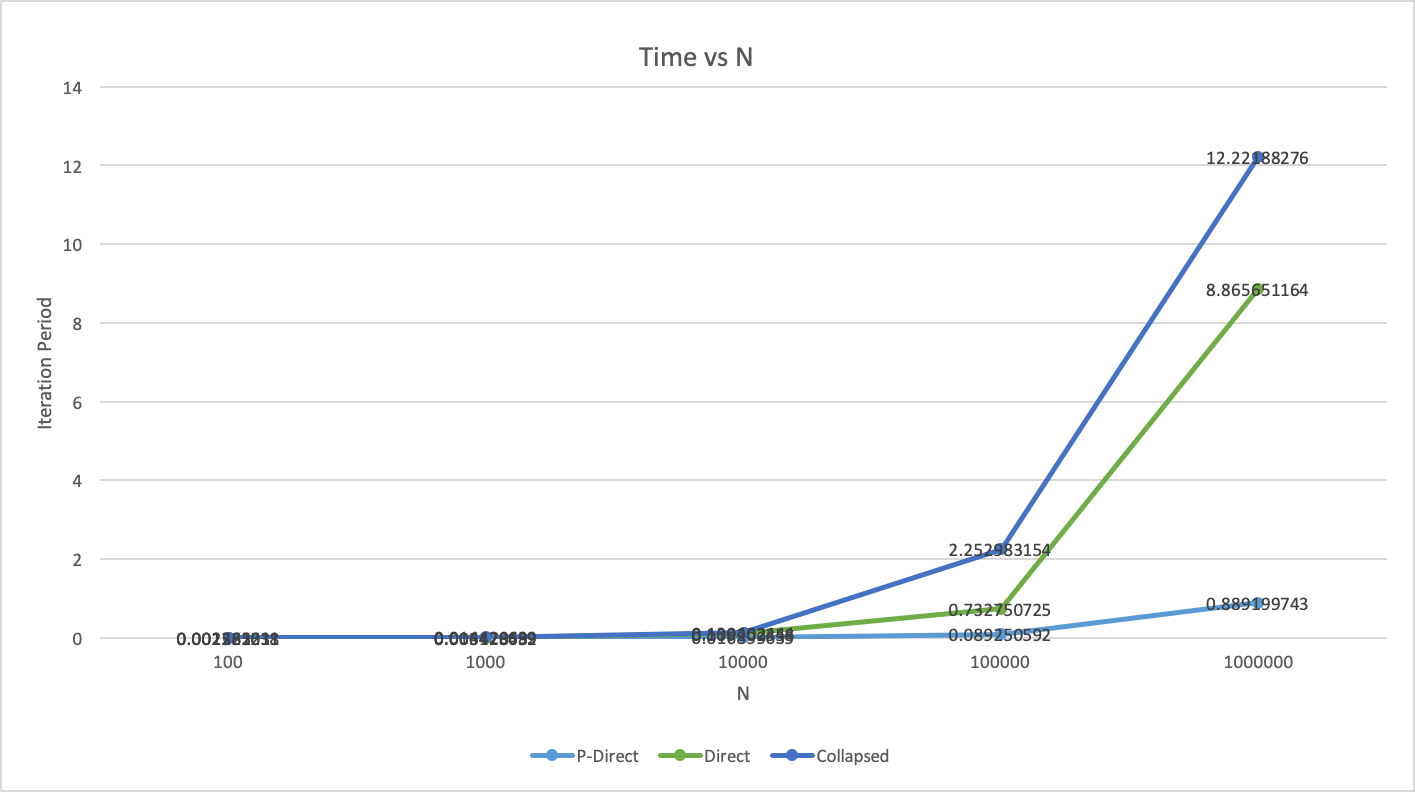
\includegraphics[width=\linewidth]{img/NVK5K5alpha1D2.png}
    \caption{$K=5, \alpha=1.0, D=2$}
  \end{subfigure}
  \hfill
  \begin{subfigure}[t]{.4\textwidth}
    \centering
    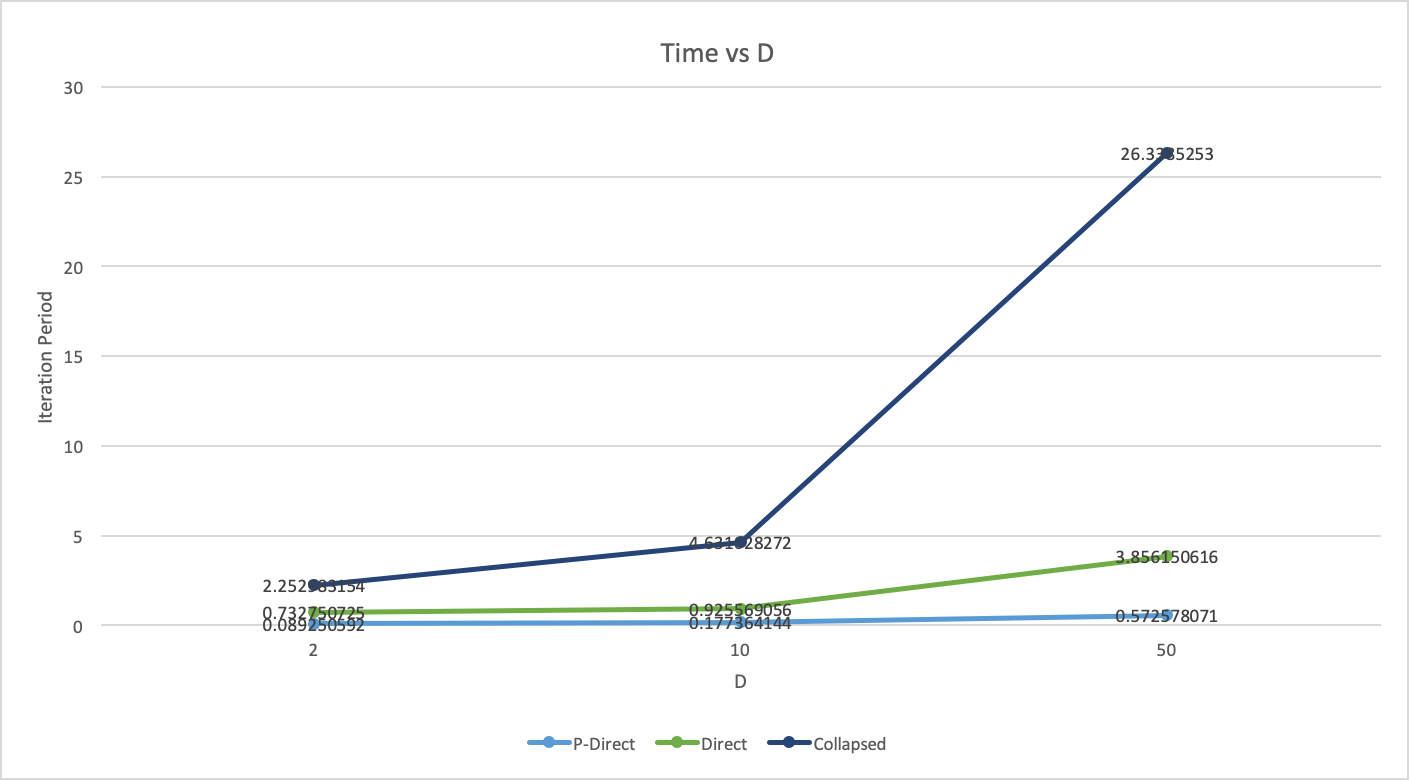
\includegraphics[width=\linewidth]{img/N100000K5K5alpha1DV.png}
     \caption{$N=100.000, K=5, \alpha=1.0$}
  \end{subfigure}

  \medskip

  \begin{subfigure}[t]{.4\textwidth}
    \centering
    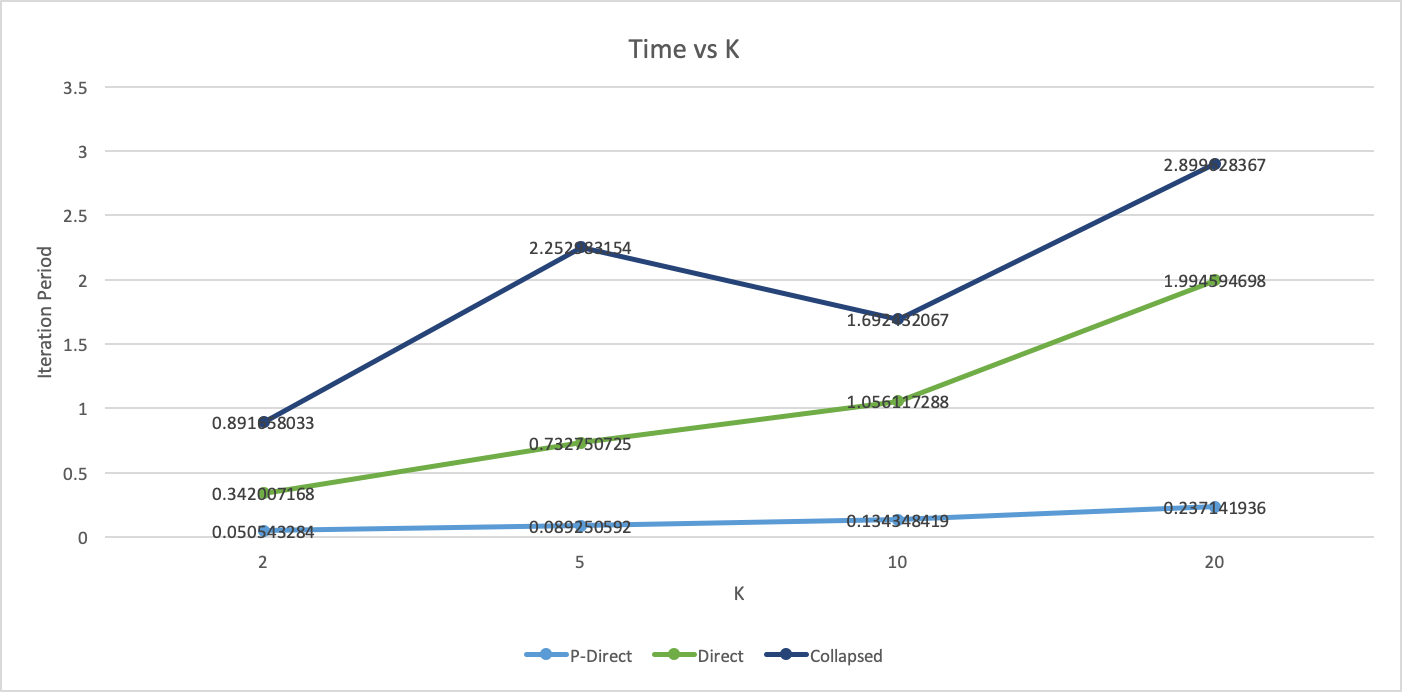
\includegraphics[width=\linewidth]{img/N100000KVKValpha1D2.png}
    \caption{$N=100.000, \alpha=1.0, D=2$}
  \end{subfigure}
  \hfill
  \begin{subfigure}[t]{.4\textwidth}
    \centering
    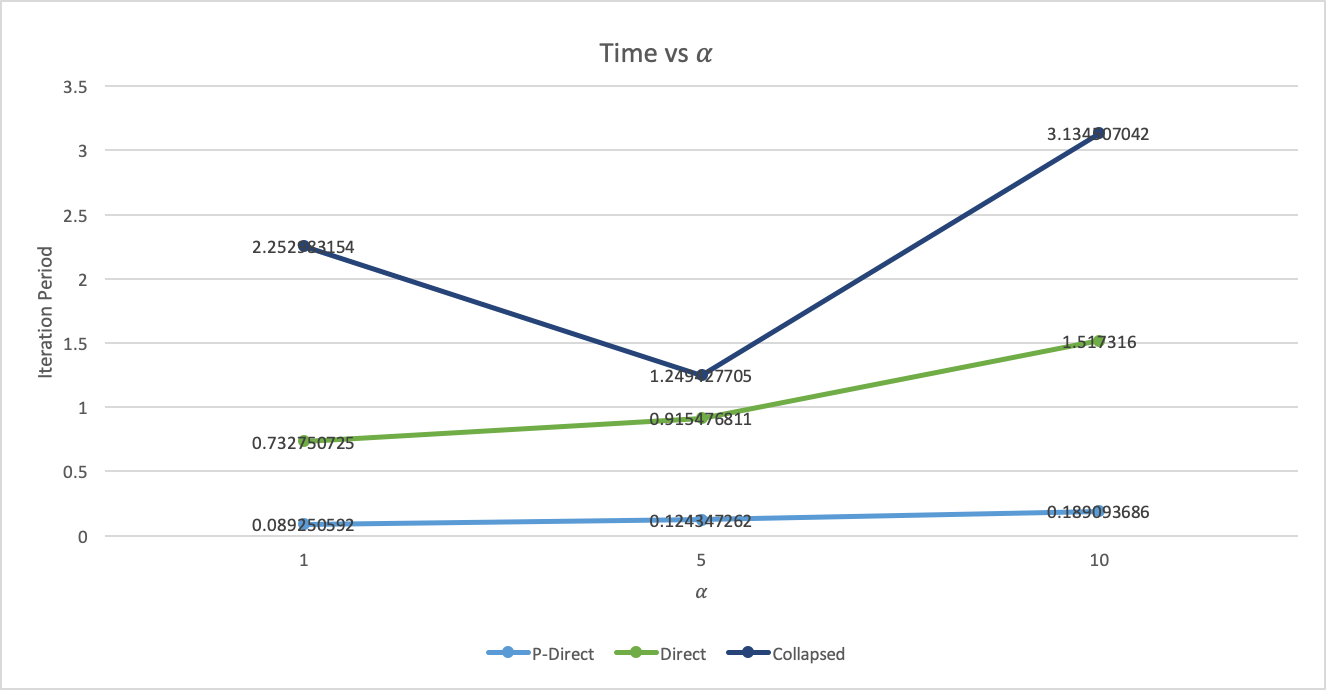
\includegraphics[width=\linewidth]{img/N100000K5K5alphaVD2.png}
     \caption{$N=100.000, K=4, D=2$}
  \end{subfigure}
\end{figure}



\subsection{Convergence Analysis}

\bibliography{cite}

\end{document}
